\documentclass[10pt,twocolumn]{article}
\usepackage[a4paper, left=1.5cm, right=1.5cm, top=2cm, bottom=3cm]{geometry}
\usepackage[T1]{fontenc}
\usepackage[utf8]{inputenc}
\usepackage[italian]{babel}
\usepackage{amsmath}
\usepackage{titling}
\usepackage{amssymb}
\usepackage{caption}
\usepackage{graphicx}
\usepackage{float}
\usepackage{relsize}
\usepackage{titlesec}
\usepackage{ragged2e}
\usepackage{circuitikz}
\usepackage{booktabs}
\usepackage{longtable}
\usepackage{makecell}
\usepackage{pdflscape}
\usepackage{enumitem}
\usepackage{tikz}
\usepackage{physics}
\usepackage{xcolor}
\usepackage[most]{tcolorbox}
\usepackage{tikz-3dplot}
\usepackage{siunitx}
\usetikzlibrary{decorations.pathmorphing}
\usetikzlibrary{arrows.meta}              % Necessario per l'opzione >=Stealth
\usepackage[colorlinks=true, linkcolor=black]{hyperref}  %per rendere l'indice genrale "interattivo"
\setlist[itemize]{itemsep=4pt, parsep=1pt}
\newtcolorbox{nota}{
  blanker,
  before skip=1em,
  after skip=1em,
  left=1em,
  borderline west={1pt}{0pt}{black},
  fontupper=\itshape,
  before upper={\noindent\textbf{Nota}:\quad}
}

% ---- Suggerimenti su cosa dire nella sezione Grafici ----
% Metti \hintsfalse per nascondere tutti i riquadri \sugg{...}
\newif\ifhints
\hintstrue
\newcommand{\sugg}[1]{%
  \ifhints
  \par\vspace{6pt}\noindent
  \fcolorbox{orange!70!black}{yellow!12}{%
    \parbox{\dimexpr\linewidth-2\fboxsep-2\fboxrule\relax}{\footnotesize\justifying\noindent\textbf{Da dire:} #1}}%
  \par\vspace{8pt}
  \fi}

\setlength{\intextsep}{8pt} % per regolare la distanza grafico tabelle
\setlength{\columnsep}{60pt}
\setlength{\tabcolsep}{4pt}

\begin{document}

    \justifying

      \title{\textbf{Misura della larghezza di una fenditura}}
      \author{Tedeschini Michele \hspace{0.7cm} Stroili Emanuele \hspace{0.7cm} Mirolo Manuele \hspace{0.7cm} Brusini Alessio}
      \date{25 novembre 2026}
      \maketitle
      \newgeometry{left=3cm, right=3cm, top=4cm, bottom=4cm}
      \onecolumn
      \tableofcontents
    \vspace{3cm}
      \begin{abstract}
        \centering
        \large


      \end{abstract}

      \newpage
    \restoregeometry
    \twocolumn
\section{Introduzione}
\section{Apparato di misura}
\section{Analisi dati}
\subsection{Grafici}
Di seguito vengono riportati grafici e commenti derivanti dall'analisi dati.
\subsubsection{Dati grezzi}
Si riportano dapprima i grafici ottenuti dal set di dati completo.
Per ottenere i grafici per l'andamento dei dati si è dapprima fatto un fit solo sulla parte centrale,
per ricavare i parametri adatti a descrivere i dati.
\paragraph{Dati del laser verde}[H]


 \begin{figure}[H]
  \centering
  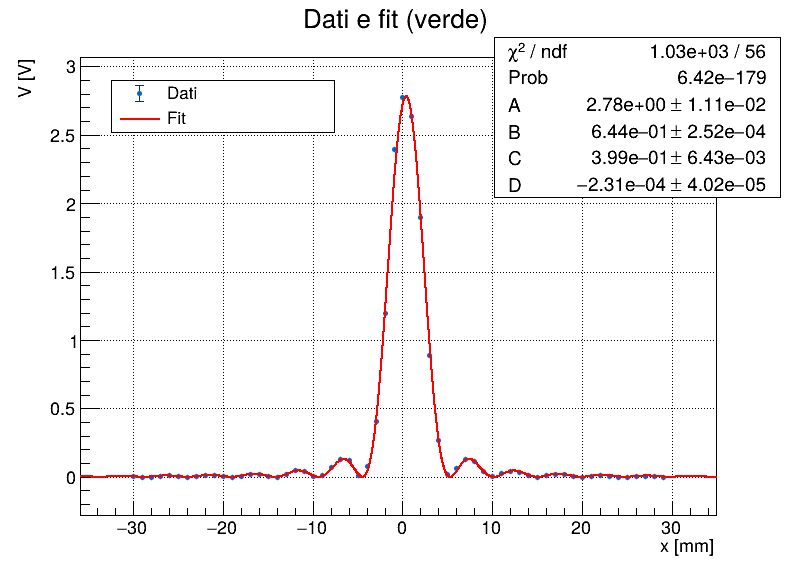
\includegraphics[width=1.0\columnwidth]{Immagini/verde/raw/verde_fit.png}
  \caption{Fit iniziale su tutti dati presi con il laser verde.}
    \label{fig:hist_manu}
 \end{figure}

 Il $\chi^2_{red}$ del fit risulta molto elevato ($\simeq 18$), il che evidenzia la difficoltà 
nel trovare un modello che descriva correttamente l'andamento dei dati. Un ulteriore prova di ciò è data
dal parametro $D$, che risulta negativo (e non compatibile con 0). Cio evidenzia il fatto che il fit 
preferisce minimizzare i dati alle code, in quanto questi hanno un errore efficace minore e contribuiscono maggiormente al $\chi^2$. 


Inserendo nel codice il limite per il parametro $D$ che esso non dovesse superare lo 0, il fit converge proprio a $D=0 mm$,
suggerendo che esso non sia converso ad un minimo, ma abbia inserito come valore il più vicino ad uno di essi.
 \begin{figure}[H]
  \centering
  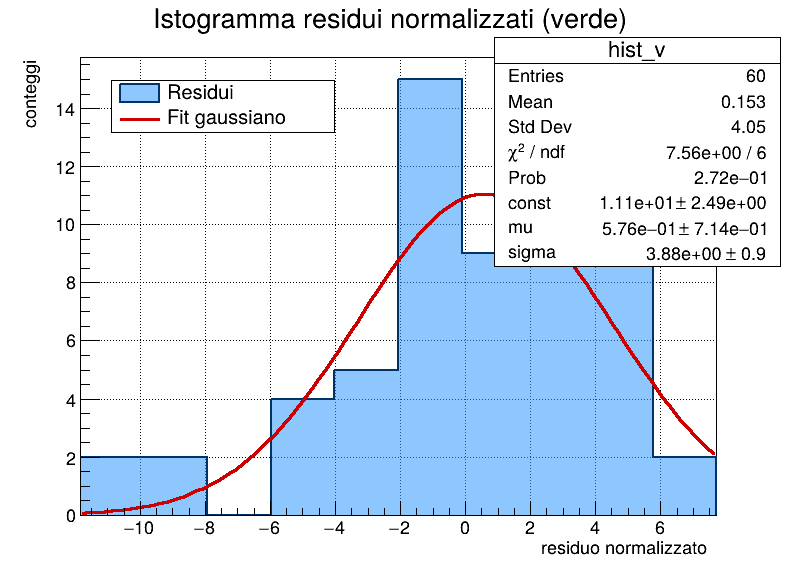
\includegraphics[width=1.0\columnwidth]{Immagini/verde/raw/verde_hist.png}
  \caption{Istogramma dei residui normalizzati ricavati dalla misura con il laser verde.}
    \label{fig:hist_manu}
 \end{figure}

 

 \begin{figure}[H]
  \centering
  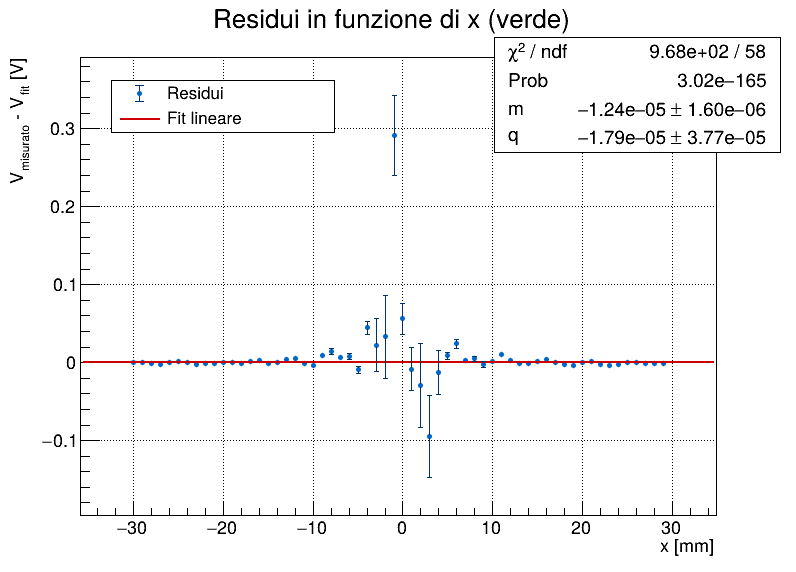
\includegraphics[width=1.0\columnwidth]{Immagini/verde/raw/verde_residui.png}
  \caption{Andamento dei residui ricavati dalla misura con il laser verde.}
    \label{fig:hist_manu}
 \end{figure}

 Anche quest'ultimo grafico conferma quanto detto prima, i dati attorno a $x = 0 mm$ 
 vengono modellati peggio rispetto a quelli sulle code.


\paragraph{Dati del laser rosso}[H]


 \begin{figure}[H]
  \centering
  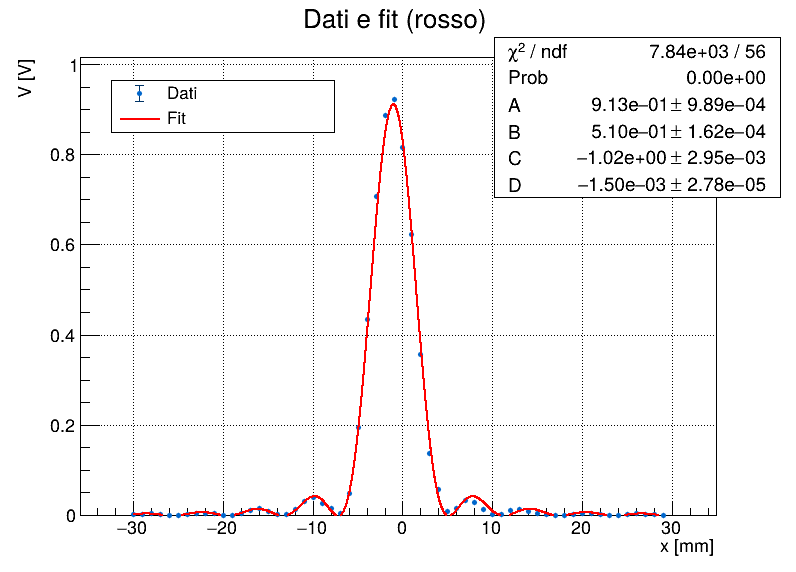
\includegraphics[width=1.0\columnwidth]{Immagini/rosso/raw/rosso_fit_nonmod.png}
  \caption{Fit iniziale su tutti dati presi con il laser rosso.}
    \label{fig:hist_manu}
 \end{figure}

  
 \begin{figure}[H]
  \centering
  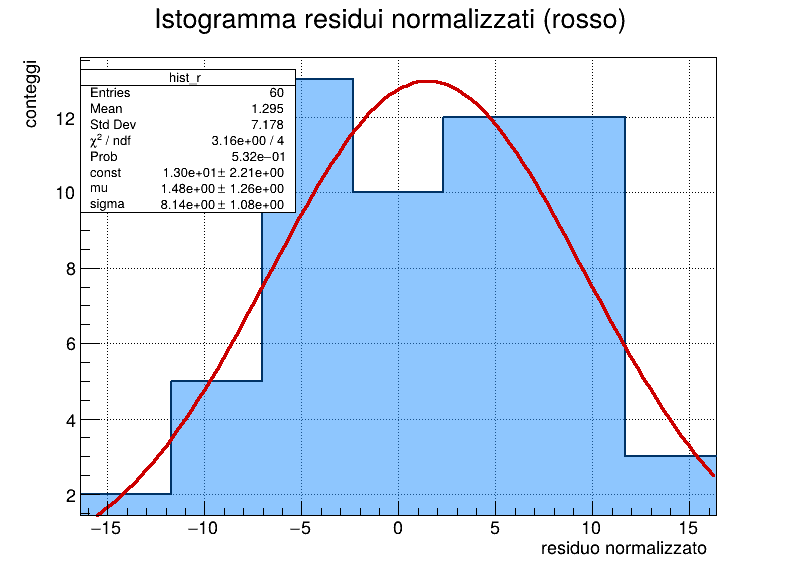
\includegraphics[width=1.0\columnwidth]{Immagini/rosso/raw/rosso_hist._nonmod.png}
  \caption{Istogramma dei residui normalizzati ricavati dalla misura con il laser rosso.}
    \label{fig:hist_manu}
 \end{figure}

 

 \begin{figure}[H]
  \centering
  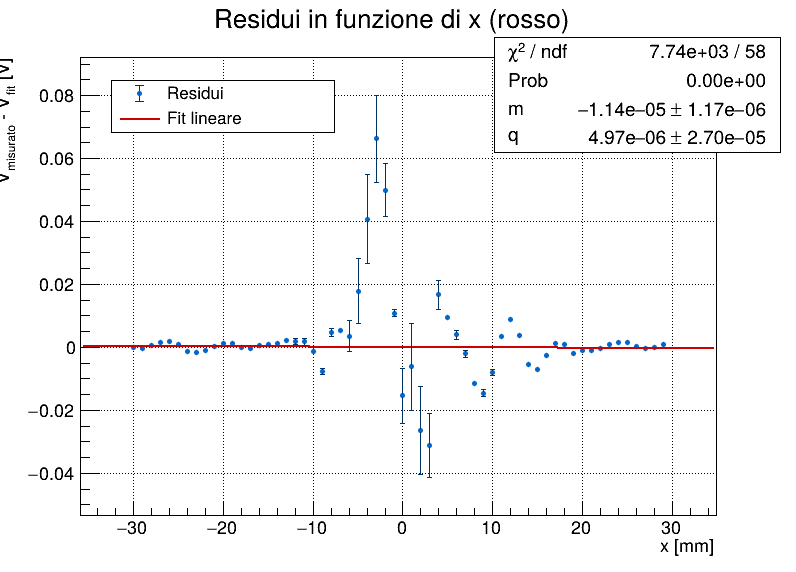
\includegraphics[width=1.0\columnwidth]{Immagini/rosso/raw/rosso_residui._nonmod.png}
  \caption{Andamento dei residui ricavati dalla misura con il laser rosso.}
    \label{fig:hist_manu}
 \end{figure}

Anche per il laser rosso abbiamo le stesse problematiche riportate antecedentemente. Inoltre, 
i residui successivi a $x=5mm$, riportano un andamento non casuale, dovuto probabilmente ad un errore
sistematico nella lettura dei dati. Infatti questo andamento è compatibile con quello di uno shift negativo 
delle misure, come visibile dalla figura sottostante.

 

 \begin{figure}[H]
  \centering
  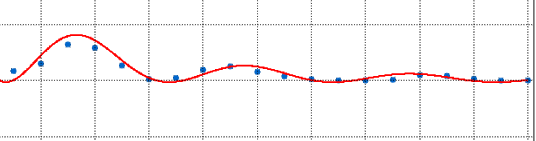
\includegraphics[width=1.0\columnwidth]{Immagini/rosso/shift_rosso.png}
  \caption{Zoom sulla parte presumibilmente traslata del dataset del laser rosso.}
    \label{fig:hist_manu}
 \end{figure}


\subsubsection{Eliminazione delle code}
Per provare a migliorare il fit, si è provato dapprima ad eliminare 5 punti dalle code dei due dataset.
Infatti, come detto prima, questi dati pesano molto nella costruzione della funzione di fit, ed essendo molto vicini 
a voltaggi nulli, traslano tutta la funzione di fit.


\paragraph{Dati del laser rosso}[H]

 \begin{figure}[H]
  \centering
  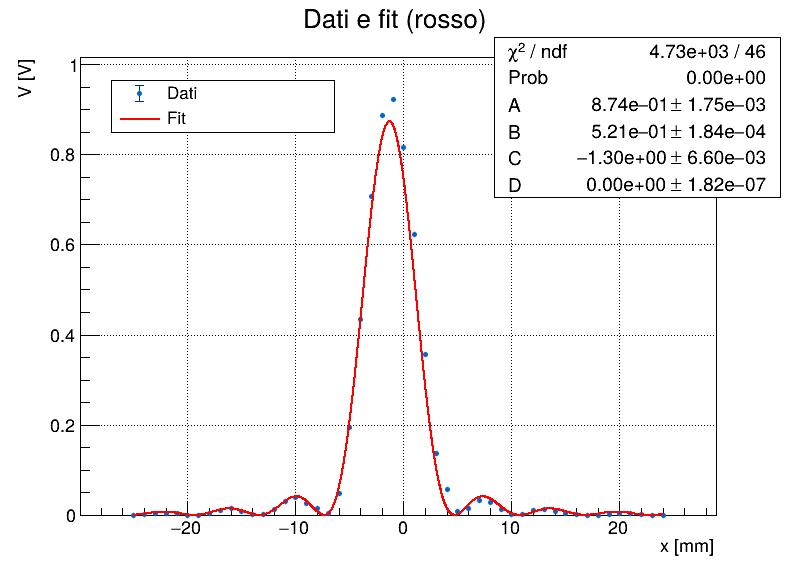
\includegraphics[width=1.0\columnwidth]{Immagini/rosso/menocode/rosso_fit._menopunti.png}
  \caption{Fit sui dati presi con il laser rosso togliendo 5 punti nelle code.}
    \label{fig:hist_manu}
 \end{figure}

\begin{figure}[H]
  \centering
  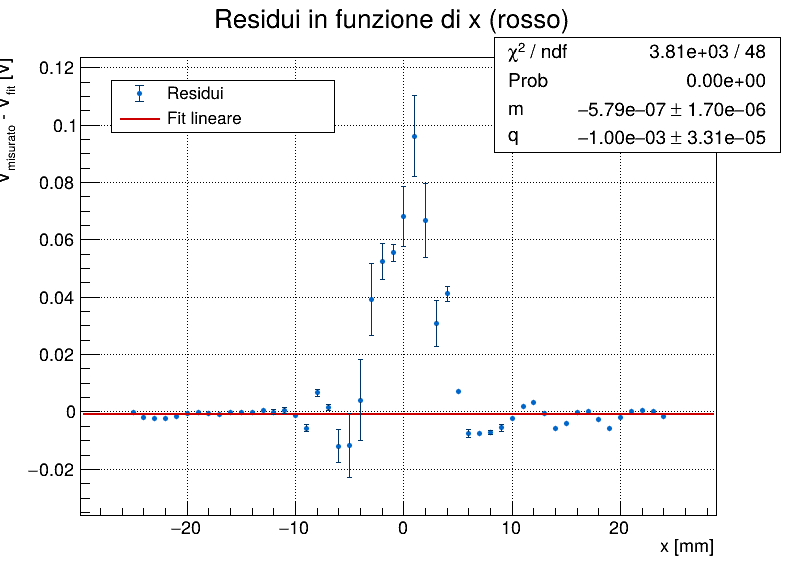
\includegraphics[width=1.0\columnwidth]{Immagini/rosso/menocode/rosso_residui_menopunti.png}
  \caption{Andamento dei residui dei dati del laser rosso togliendo 5 punti nelle code.}
    \label{fig:hist_manu}
 \end{figure}

 \paragraph{Dati del laser verde}[H]

 \begin{figure}[H]
  \centering
  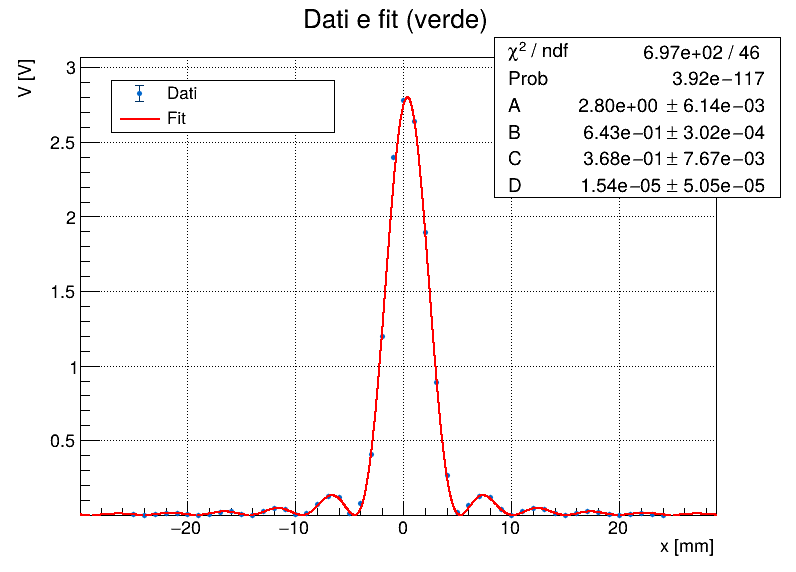
\includegraphics[width=1.0\columnwidth]{Immagini/verde/menocode/verde_fit_menopunti.png}
  \caption{Fit sui dati presi con il laser verde togliendo 5 punti nelle code.}
    \label{fig:hist_manu}
 \end{figure}

 \begin{figure}[H]
  \centering
  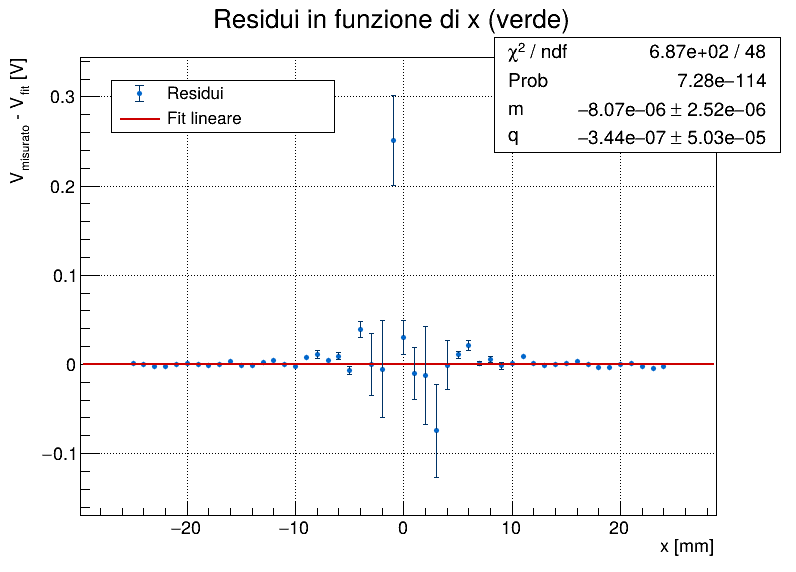
\includegraphics[width=1.0\columnwidth]{Immagini/verde/menocode/verde_residui_menopunti.png}
  \caption{Andamento dei residui dei dati del laser verde togliendo 5 punti nelle code.}
    \label{fig:hist_manu}
 \end{figure}

 Da quest'ultimo grafico è evidente che il fit ha un andamento nettamente migliore rispetto a prima. 
 Molti dei residui centrali risultano ora compatibili con la retta a pendenza nulla attesa.


\subsubsection{Divisione del fit}

\paragraph{Laser rosso}[H]

  \begin{figure}[H]
    \centering
    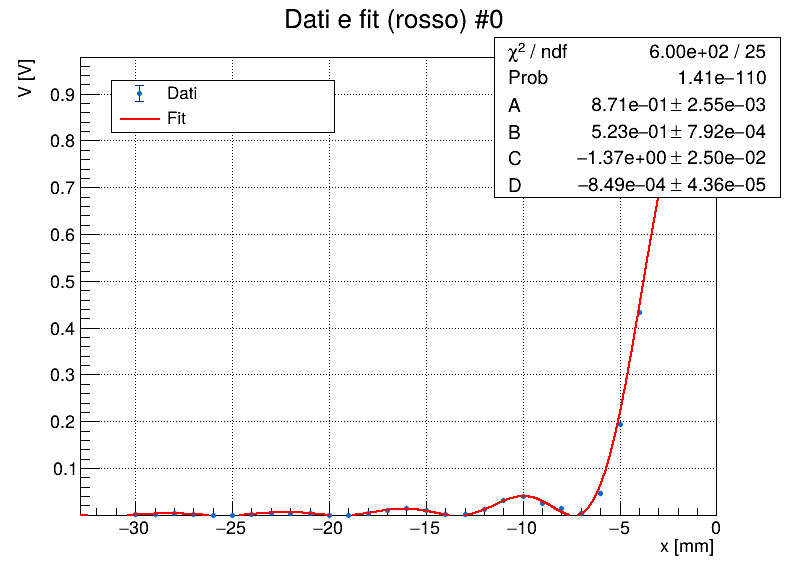
\includegraphics[width=1.0\columnwidth]{Immagini/rosso/fit_parziale_rosso_0.png}
    \caption{Prima parte del fit sui dati del laser rosso togleindo 5 punti delle code.}
      \label{fig:hist_manu}
  \end{figure}

  \begin{figure}[H]
    \centering
    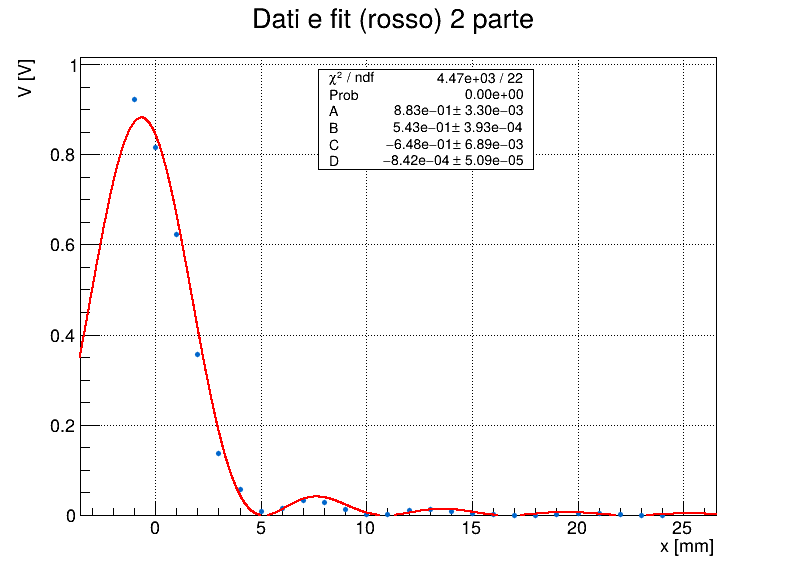
\includegraphics[width=1.0\columnwidth]{Immagini/rosso/fit_parziale_rosso_1.png}
    \caption{Seconda parte del fit sui dati del laser rosso togleindo 5 punti delle code.}
      \label{fig:hist_manu}
  \end{figure}

\paragraph{Laser verde}[H]

  \begin{figure}[H]
    \centering
    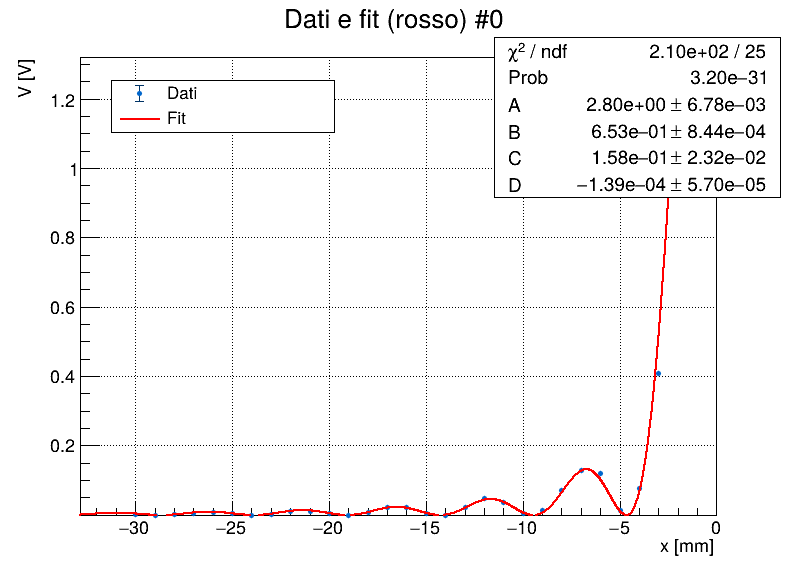
\includegraphics[width=1.0\columnwidth]{Immagini/verde/fit_parziale_verde_0.png}
    \caption{Prima parte del fit sui dati del laser verde togleindo 5 punti delle code.}
      \label{fig:hist_manu}
  \end{figure}

  \begin{figure}[H]
    \centering
    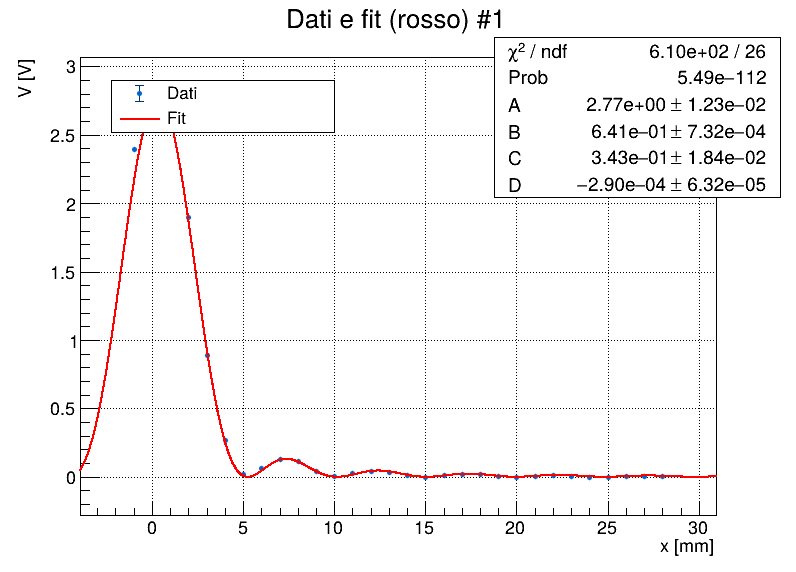
\includegraphics[width=1.0\columnwidth]{Immagini/verde/fit_parziale_verde_1.png}
    \caption{Seconda parte del fit sui dati del laser verde togleindo 5 punti delle code.}
      \label{fig:hist_manu}
  \end{figure}

\subsubsection{Aggiunta di un offset ai dati del laser rosso}

  \begin{figure}[H]
    \centering
    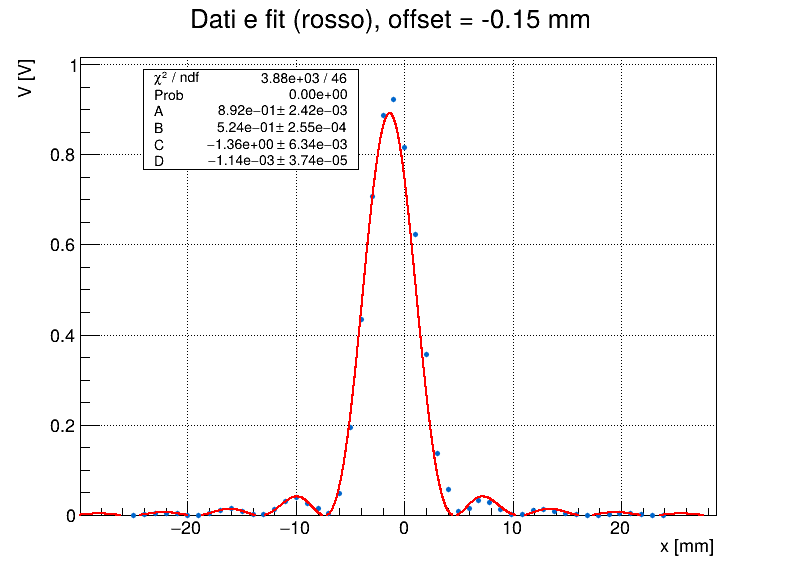
\includegraphics[width=1.0\columnwidth]{Immagini/rosso/shift/shit_da_32/rosso_fit_best_offset.png}
    \caption{Fit sui dati del laser rosso (togliendo i punti delle code), aggiungendo un offset.}
      \label{fig:hist_manu}
  \end{figure}

  d verde = 0.22003686339291917 ± 0.0005543561988560995 mm
d rosso = 0.21892251178281713 ± 0.000552277336286421 mm
|d verde - d rosso| = 0.0011143516101020379 mm  (1.42 sigma)
d verde è compatibile con d rosso

  \begin{figure}[H]
    \centering
    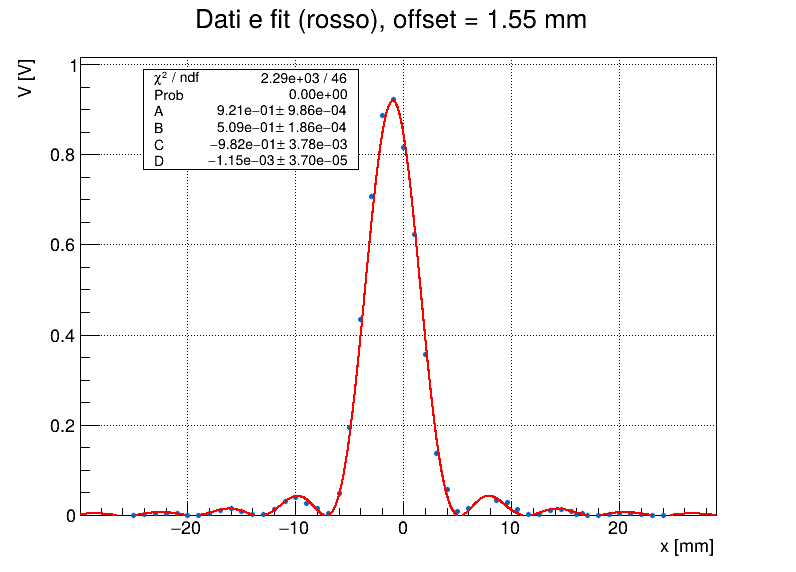
\includegraphics[width=1.0\columnwidth]{Immagini/rosso/shift/shif_32_41/rosso_fit_best_offset.png}
    \caption{Fit sui dati del laser rosso (togliendo i punti delle code), aggiungendo un offset.}
      \label{fig:hist_manu}
  \end{figure}

  d verde = 0.22003686339291917 ± 0.0005543561988560995 mm
d rosso = 0.21254465869553069 ± 0.0005318222122972024 mm
|d verde - d rosso| = 0.007492204697388483 mm  (9.75 sigma)
d verde NON è compatibile con d rosso


  \begin{figure}[H]
    \centering
    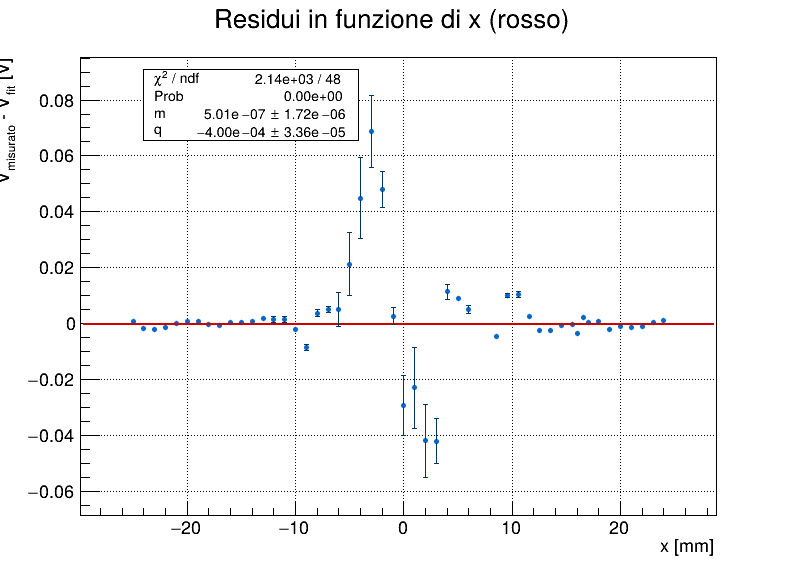
\includegraphics[width=1.0\columnwidth]{Immagini/rosso/shift/shif_32_41/rosso_residui.png}
    \caption{Fit sui dati del laser rosso (togliendo i punti delle code), aggiungendo un offset.}
      \label{fig:hist_manu}
  \end{figure}




\section{Conclusioni}
\end{document}